\documentclass[12pt]{article}
\usepackage{amsmath, amssymb} 
\usepackage{graphicx}

%Code settings
\usepackage{listings}
\usepackage{xcolor}

\definecolor{vscode-bg}{RGB}{255,255,255} % White background
\definecolor{vscode-fg}{RGB}{30,30,30}    % Dark foreground
\definecolor{vscode-keyword}{RGB}{86,156,214}
\definecolor{vscode-comment}{RGB}{87,166,74}
\definecolor{vscode-string}{RGB}{214,157,133}

\lstdefinestyle{vscode-c}{
    backgroundcolor=\color{vscode-bg},
    basicstyle=\color{vscode-fg}\scriptsize\ttfamily,
    keywordstyle=\color{vscode-keyword},
    commentstyle=\color{vscode-comment},
    stringstyle=\color{vscode-string},
    showstringspaces=false,
    breaklines=true,
    breakatwhitespace=true,
    tabsize=4,
    captionpos=b,
    frame=single,
    framexleftmargin=5mm,
    framextopmargin=2mm,
    framexbottommargin=2mm,
    framexrightmargin=5mm,
    xleftmargin=2mm,
    xrightmargin=1mm,
    aboveskip=3mm,
    belowskip=3mm,
}

\lstset{style=vscode-c}


\title{The shortest physical path to victory in "Mensch ärgere Dich nicht"}
\author{Erik Seewald}
\date{\today}

\begin{document}
\maketitle

\tableofcontents

\newpage

\section{Introduction}

\subsection{The game}

"Mensch ärgere Dich nicht" is a very popular board game in Germany, derived from the Indian "Pachisi" and the English "Ludo".
It was introduced early in the 20th century and has since enjoyed a comfortable life in the cupboard and occasionally on the table
of every German family.

\begin{figure}[htbp]
    \centering
    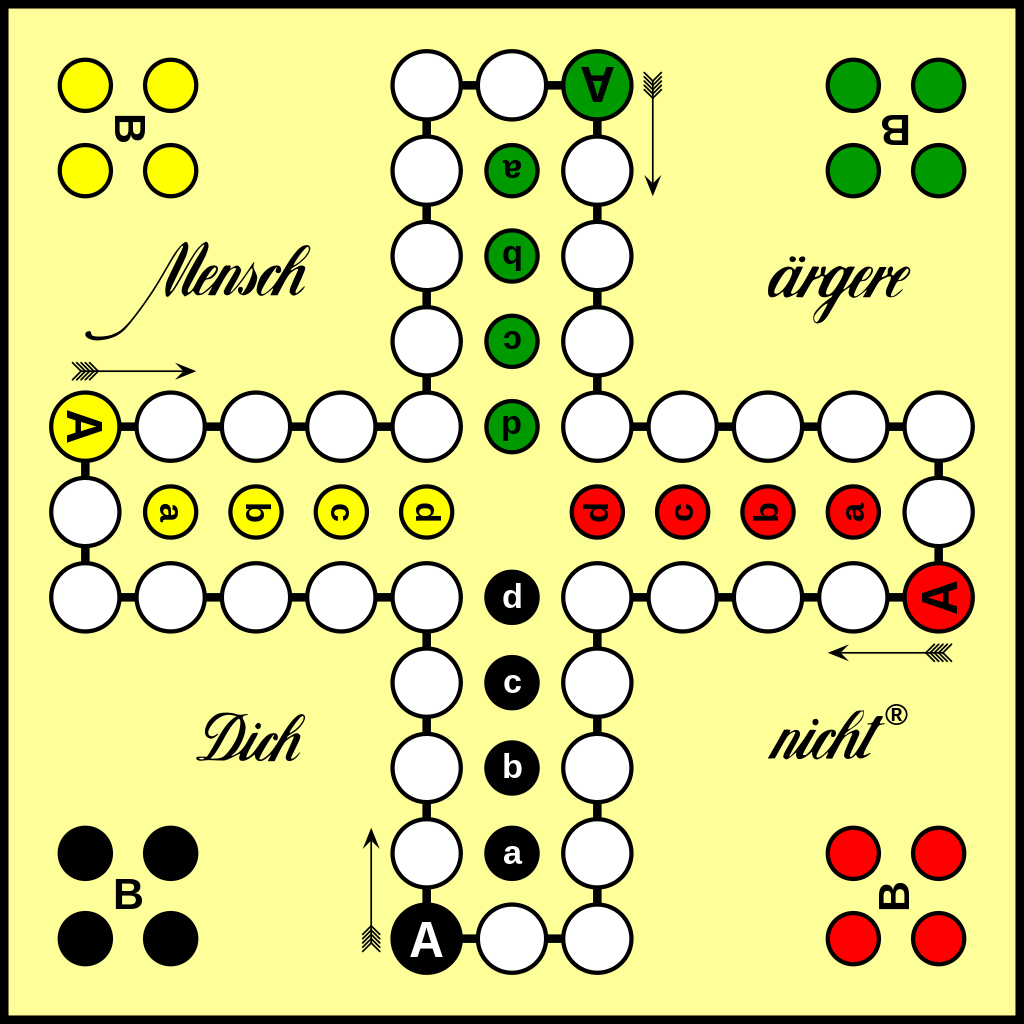
\includegraphics[width=0.7\textwidth]{images/Figure1}
    \caption{The board}
    \label{fig:board}
\end{figure}


The board is made up of 72 tiles - of which 48 are relevant to any single player.
There are four color-coded fields, each consisting of four tiles and labeled with a capital 'B' in the corners of the board. These fields serve as the starting positions for each player's four pieces. At the start of the game every piece is stuck here until a 6 is rolled, any other number will result in a null turn. These 4 tiles with be referred to as the "\textbf{purgatory}". However, when a player rolls a six, they are allowed to move one piece onto their respective color-coded starting tile, marked with a capital 'A'. Here an arrow indicates the starting direction. 
The main playing field consists of 40 tiles, mostly white and connected by black lines.
Here a player needs to move towards making a full loop around the plus-shaped field as fast as possible.
When a roll results in a number that would place a piece on or beyond the starting tile, the piece instead advances to the color-coded '\textbf{abcd-tiles}', which will be consistently referred to as such. These tiles represent the goal for each piece.
The letter a piece lands on is irrelevant. The game is finished when one player has filled out all of their \textbf{abcd-tiles}.

The frustrating mechanic that contributes to the game's iconic title arises from the interactions among different players. If a roll results in a piece moving onto a tile occupied by an opponent's piece, the occupying piece is knocked out and must return to the \textbf{purgatory}.
However, if a piece lands on a tile occupied by another piece of the same team, the turn is nullified.

These straightforward yet entertaining rules have contributed to the game's enduring popularity across generations. However, for our current objective, we will disregard its fundamental core—player interaction—completely.



\subsection{The problem}
Based on the rules of the game it is easy to assume that the quickest way to win would be to constantly roll a 6.
But what if we do not care about the "quickest" way and instead focus on the "shortest" way?
Every piece needs to be moved to it's new rolled position, but there is no rule requiring that movement to follow the path.
Instead, often, players will just move the piece in a straight line towards a tile and thereby skipping a large piece of the path. 

\begin{figure}[htbp]
    \centering
    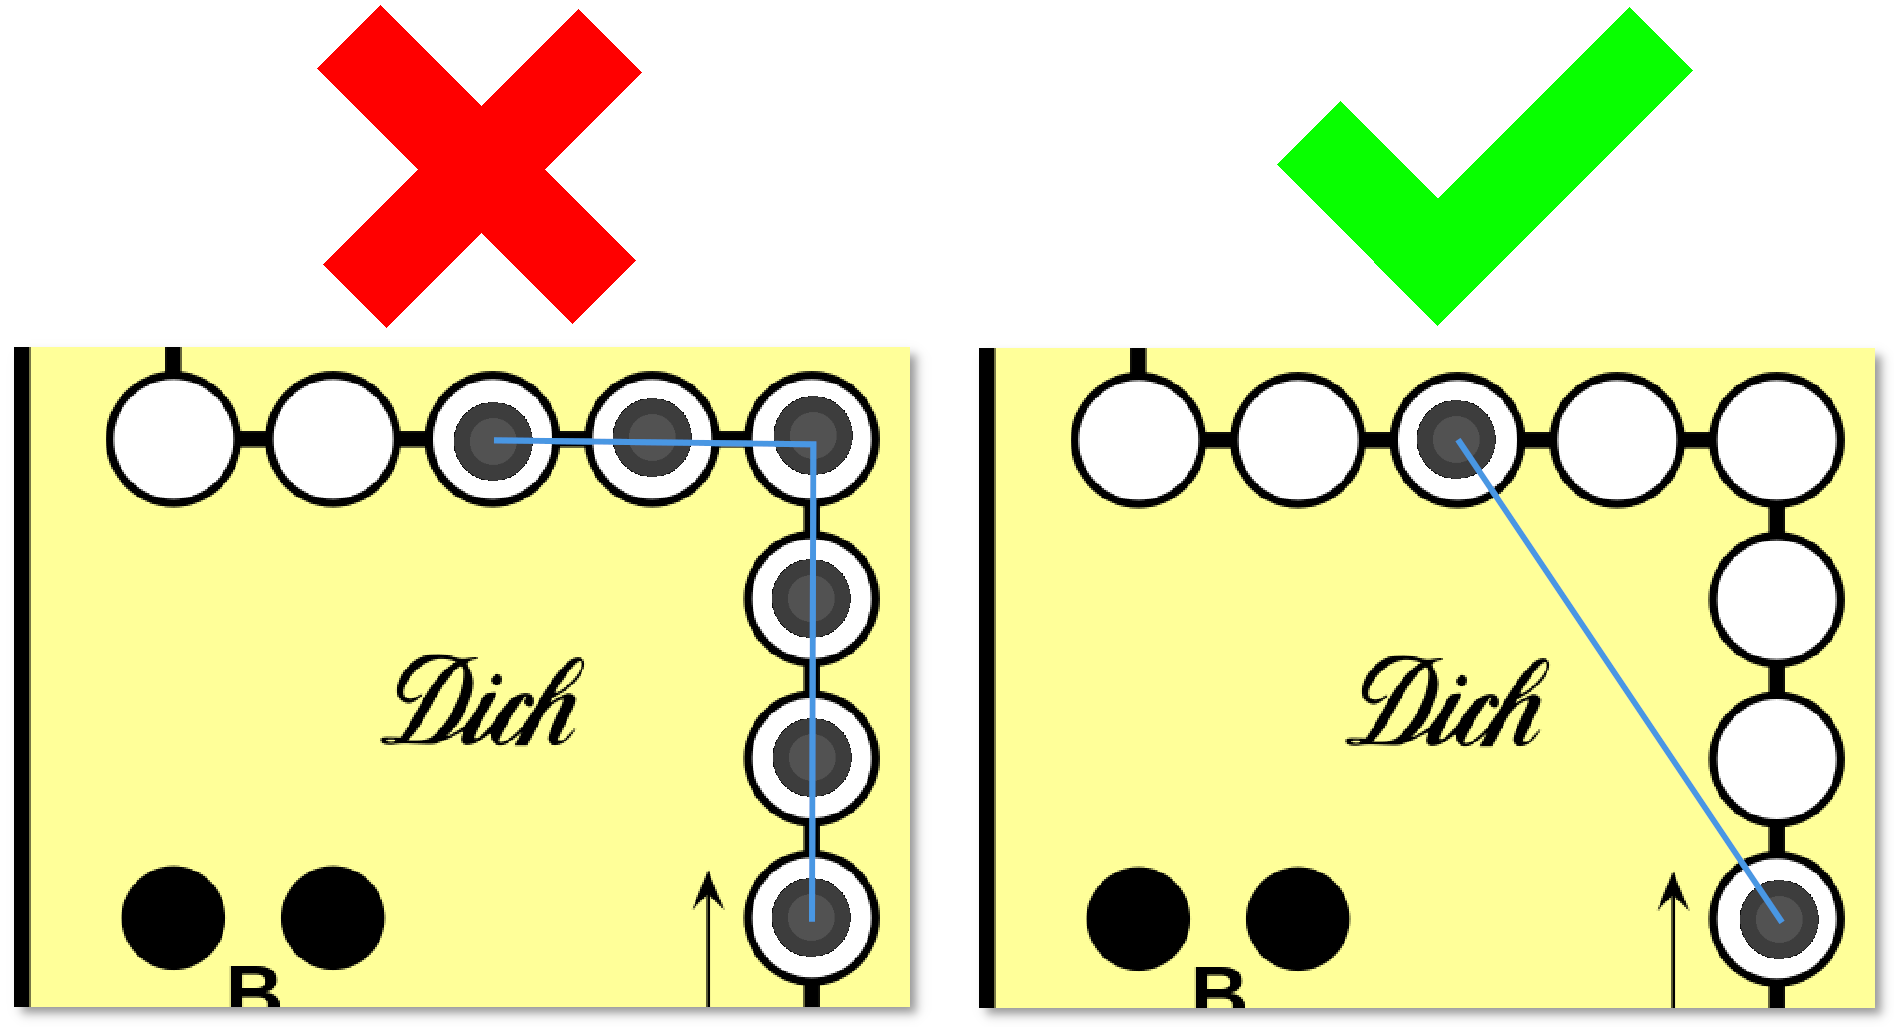
\includegraphics[width=0.6\textwidth]{images/Figure2}
    \caption{Shortcuts}
    \label{fig:shortcuts}
\end{figure}

One could wonder about the minimum amount of physical movement required to win a game if every roll is optimized towards skipping the maximum amount of tiles in a straight path. Since we only want to find the absolute best case scenario, we can completely ignore the other players. Ideally they never roll a 6 and stay in \textbf{purgatory} forever.


\section{Computability}\label{sec:computability}
The goal is to make a program that finds the shortest path fitting our description. Let us take a closer look into what kind of challenges this task will provide and what variables need to be accounted for.

Before even beginning to think about writing a program we need to assure ourselves that the problem is conceptually computable within a reasonable time frame.
The naive approach would be to simply loop through every possible outcome of the game and compare the length of all the paths
taken.
Every turn there are 6 different numbers that can be rolled. Additionally, for each of these 6 numbers there are 4 different outcomes depending on which piece the player chooses to move.
\[
    N_{Outcomes~per~turn} = 6_{Different~rolls} \cdot 4_{Pieces} = 24
\]
Of course, once some of the pieces are finished and can no longer move, N will change. This will be ignored for now however.

The number of turns to finish a game, when ignoring other players, can be assumed to be 4 times the amount needed for a single piece to finish. For simplicity's sake we can assume that average amount of turns for one piece will be the number of tiles divided by the average roll. When combining both of these terms we need to finish by rounding up to the next highest integer.
\[
    T_{Number~of~turns} =  \lceil \frac{44_{Tiles}}{3_{Average~Roll}} \cdot 4_{Pieces} \rceil
    =  59
\]

For each of the N outcomes per turn there will be N new outcomes, for which there will be N outcomes again and so forth until the game is finished after about T iterations. That means the amount of positions that need to be checked to find the shortest path via the naive approach would be N times N times N times N.... until all pieces are finished, in other words, N raised to T. Recall that we are ignoring the change in N resulting from less pieces being available to choose from over time.
\[
    P_{Positions} =  N^T = 24^{59} = 2.70684421 \cdot 10^{81}
\]

As you can see, this is a horrendously large number. In fact, it can be compared to the amount of particles in our universe, which is estimated to be around $10^{78}$ to $10^{82}$. Clearly, the naive approach will not work.

One way to improve upon this method would be decreasing N. Luckily, there is actually no reason to even consider which of the 4 pieces to move each turn, as the position of one piece can never be beneficial to another of the same team. This means we can safely only move on piece towards it's goal at a time and thereby get rid of the factor 4 in the equation for N.
\[
    N_{Outcomes~per~turn} = 6_{Different~rolls}
\]
\[
    P_{Positions} =  N^T = 6^{59} =8.145613\ \cdot 10^{45}
\]

This is a lot better but still way out of the range of easy computability.
However, N is not the only number that can be decreased by ignoring piece interaction. We can separate each of the 4 pieces' laps around the board into discrete problems to solve by having one piece on the main board at a time and the others either in \textbf{purgatory} or on the \textbf{abcd-tiles}.
\[
    S_{Purgatory} = 4_{Pieces} - F_{abcd}
\]
That means the problem boils down to finding the 4 shortest paths from the starting position to each of the 4 \textbf{abcd-tiles}.
Therefore we can remove the multiplication by the number of pieces from T and instead add it to the term for P.
\[
    T_{Turns~per~piece} =  \lceil \frac{44_{Tiles}}{3_{Average~Roll}}\rceil
    =  15
\]
\[
    P_{Number~of~positions} =  4_{Pieces} \cdot N^T = 4 \cdot 6^{15} = 1.88073994 \cdot 10^{12}
\]
P now seems computable. If we were able to write a program that can check 10 million positions in a second, it would take about
52 hours to complete. This will be optimized further of course, but for now we can be assured that the problem can actually be solved.


\section{Solving the problem}

\subsection{The idea}
The goal is to construct a program that is capable of not only finding the shortest path, but also doing so within a reasonable time-frame. Therefore it is best to begin by getting an overview over all the requirements such a program must fulfill and how they could conceptually be implemented. Let us begin by specifying a few constants to work with from now on. Since there is no constant agreed upon measurement for Mensch-ärgere-Dich-nicht boards, the program will be working with measurements generalized as "units".
\begin{itemize}
    \item The board size will be 10,000x10,000 units.
    \item The distance between two adjacent tiles on the main board will always be 850 units.
    \item The program will assume the role of player black, putting it's starting position A at (4170, 9170). Here (0,0) lies at the top left of the board.
\end{itemize}

Ideally the program should calculate all distances ahead of time so they can simply be looked up in a table while the shortest path is being searched. That may sound like a very large table at first, but any one tile only needs to calculate the distance to 6 neighbors as any distance to tiles further than 6 away will never be necessary when playing with a normal die. Therefore our list would not be longer than 40 tiles times 6 neighbors, or 240 entries. It is definitely more efficient to save 240 entries once and then looking them up instead of doing millions or billions of the same calculation over and over again while different positions are being searched through.

Additionally, the one set of distances that can be guaranteed to be included in the shortest path are those required to move each piece to the starting position. Since the tiles in the \textbf{purgatory} are (3,0), (4,0), (3,1), (4,1) tiles away from tile A and the tile distance is 850 units, the minimum total movement to the starting position when rounded up is:

\[
	\lceil 3\cdot850\ +\ 4\cdot850\ +\ \sqrt{\left(3\cdot850\right)^{2}+850^{2}}+\ \sqrt{\left(4\cdot850\right)^{2}+850^{2}}\rceil = 12143
\]

\newpage

Now we can begin specifying the conceptual program structure.
There should be a main loop that calls a function to find the shortest path for each of the 4 starting positions to their respective \textbf{abcd-tile} and then adds them up together.

\begin{figure}[htbp]
    \centering
    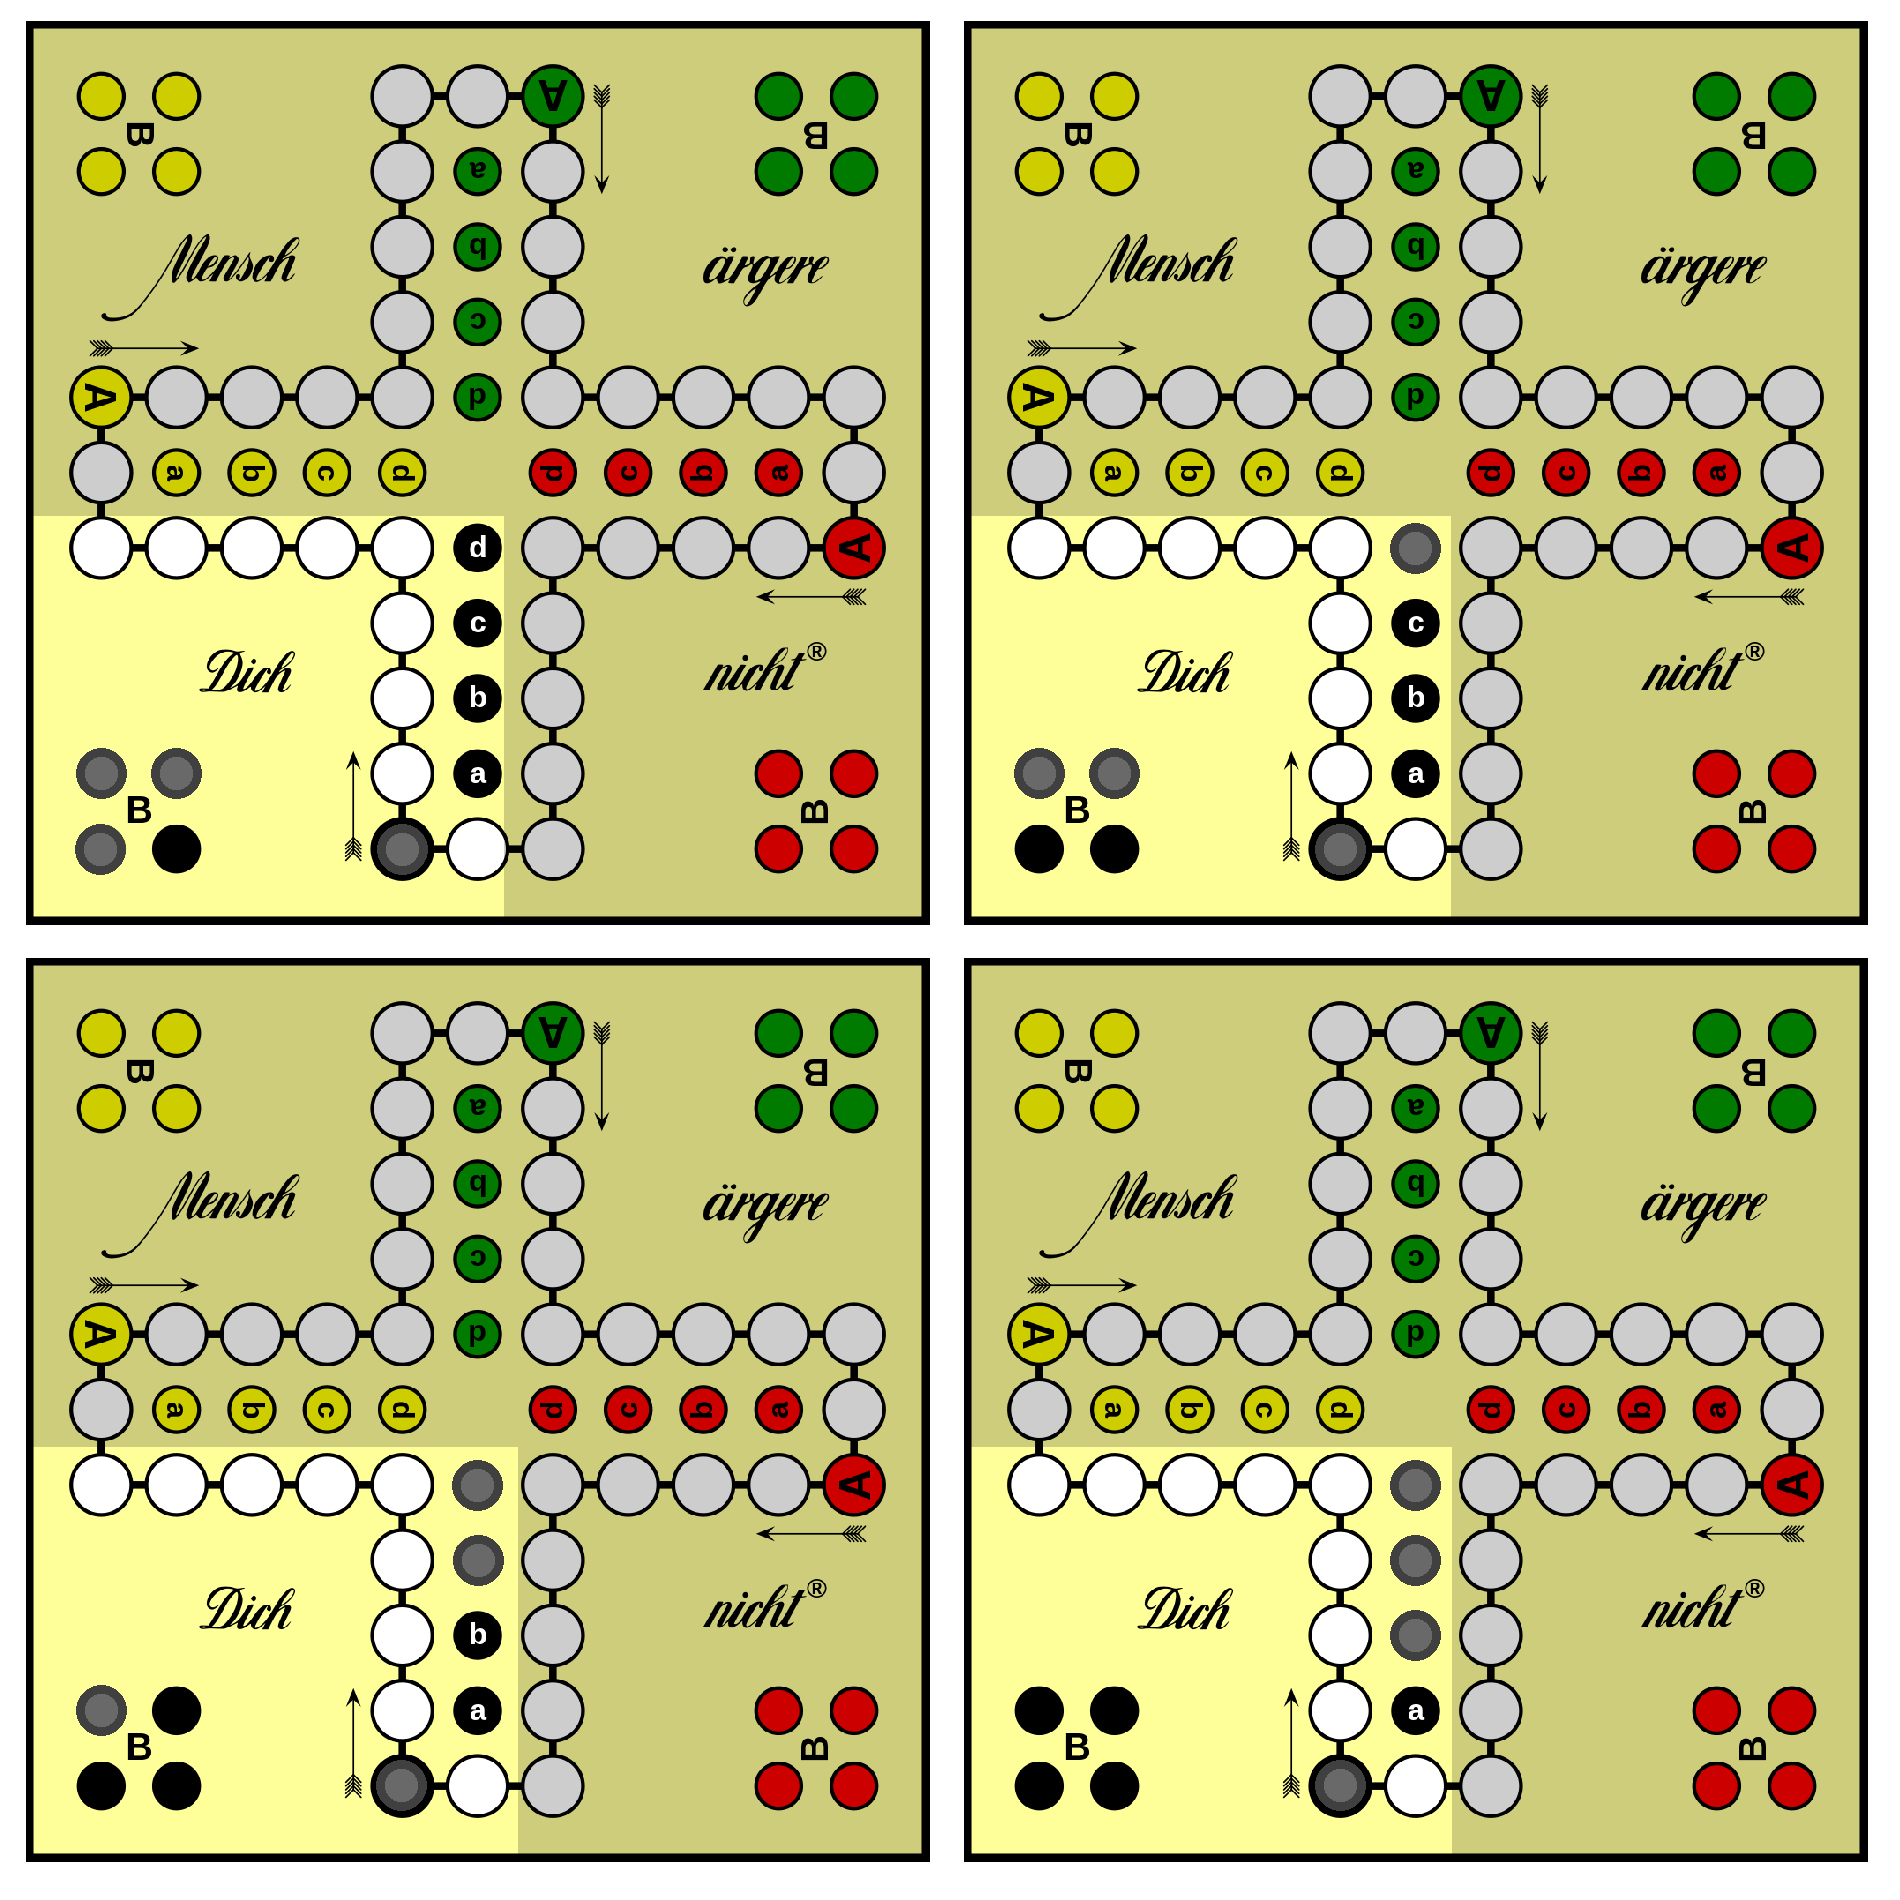
\includegraphics[width=0.6\textwidth]{images/Figure3}
    \caption{Starting positions}
    \label{fig:startpos}
\end{figure}

The reason for filling up the \textbf{abcd-tiles} starting from d at the very back is to prevent pieces from getting in the way of each other and thereby blocking the shortest path.

\begin{figure}[htbp]
    \centering
    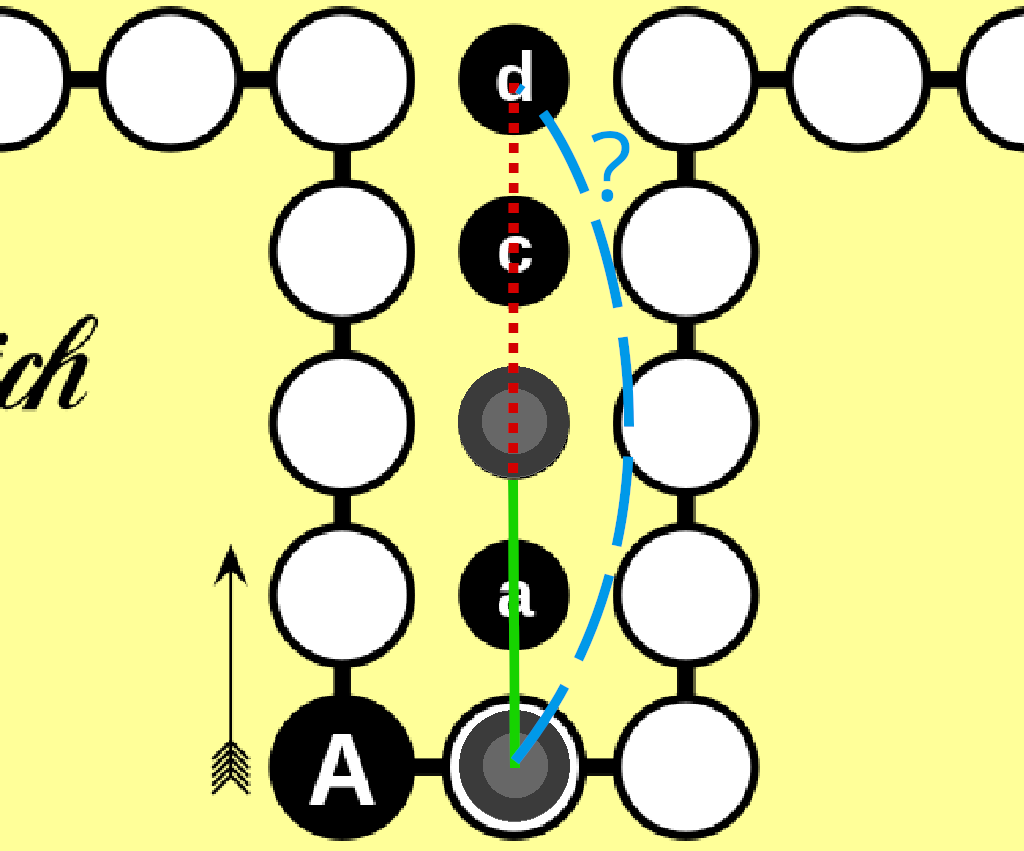
\includegraphics[width=0.3\textwidth]{images/Figure4}
    \caption{Blocked path}
    \label{fig:blockedpath}
\end{figure}

\newpage

The function finding the shortest path for a single starting position should operate recursively. It should take a specific position as well as the distance moved towards that position so far and then call itself six times and thereby looping over it's "\textbf{sub-trees}".
A \textbf{sub-tree} in this context is simply all the positions that follow a specific roll from a specific position when the total series of possible choices is imagined as a tree with it's roots at the starting position.

\begin{figure}[htbp]
    \centering
    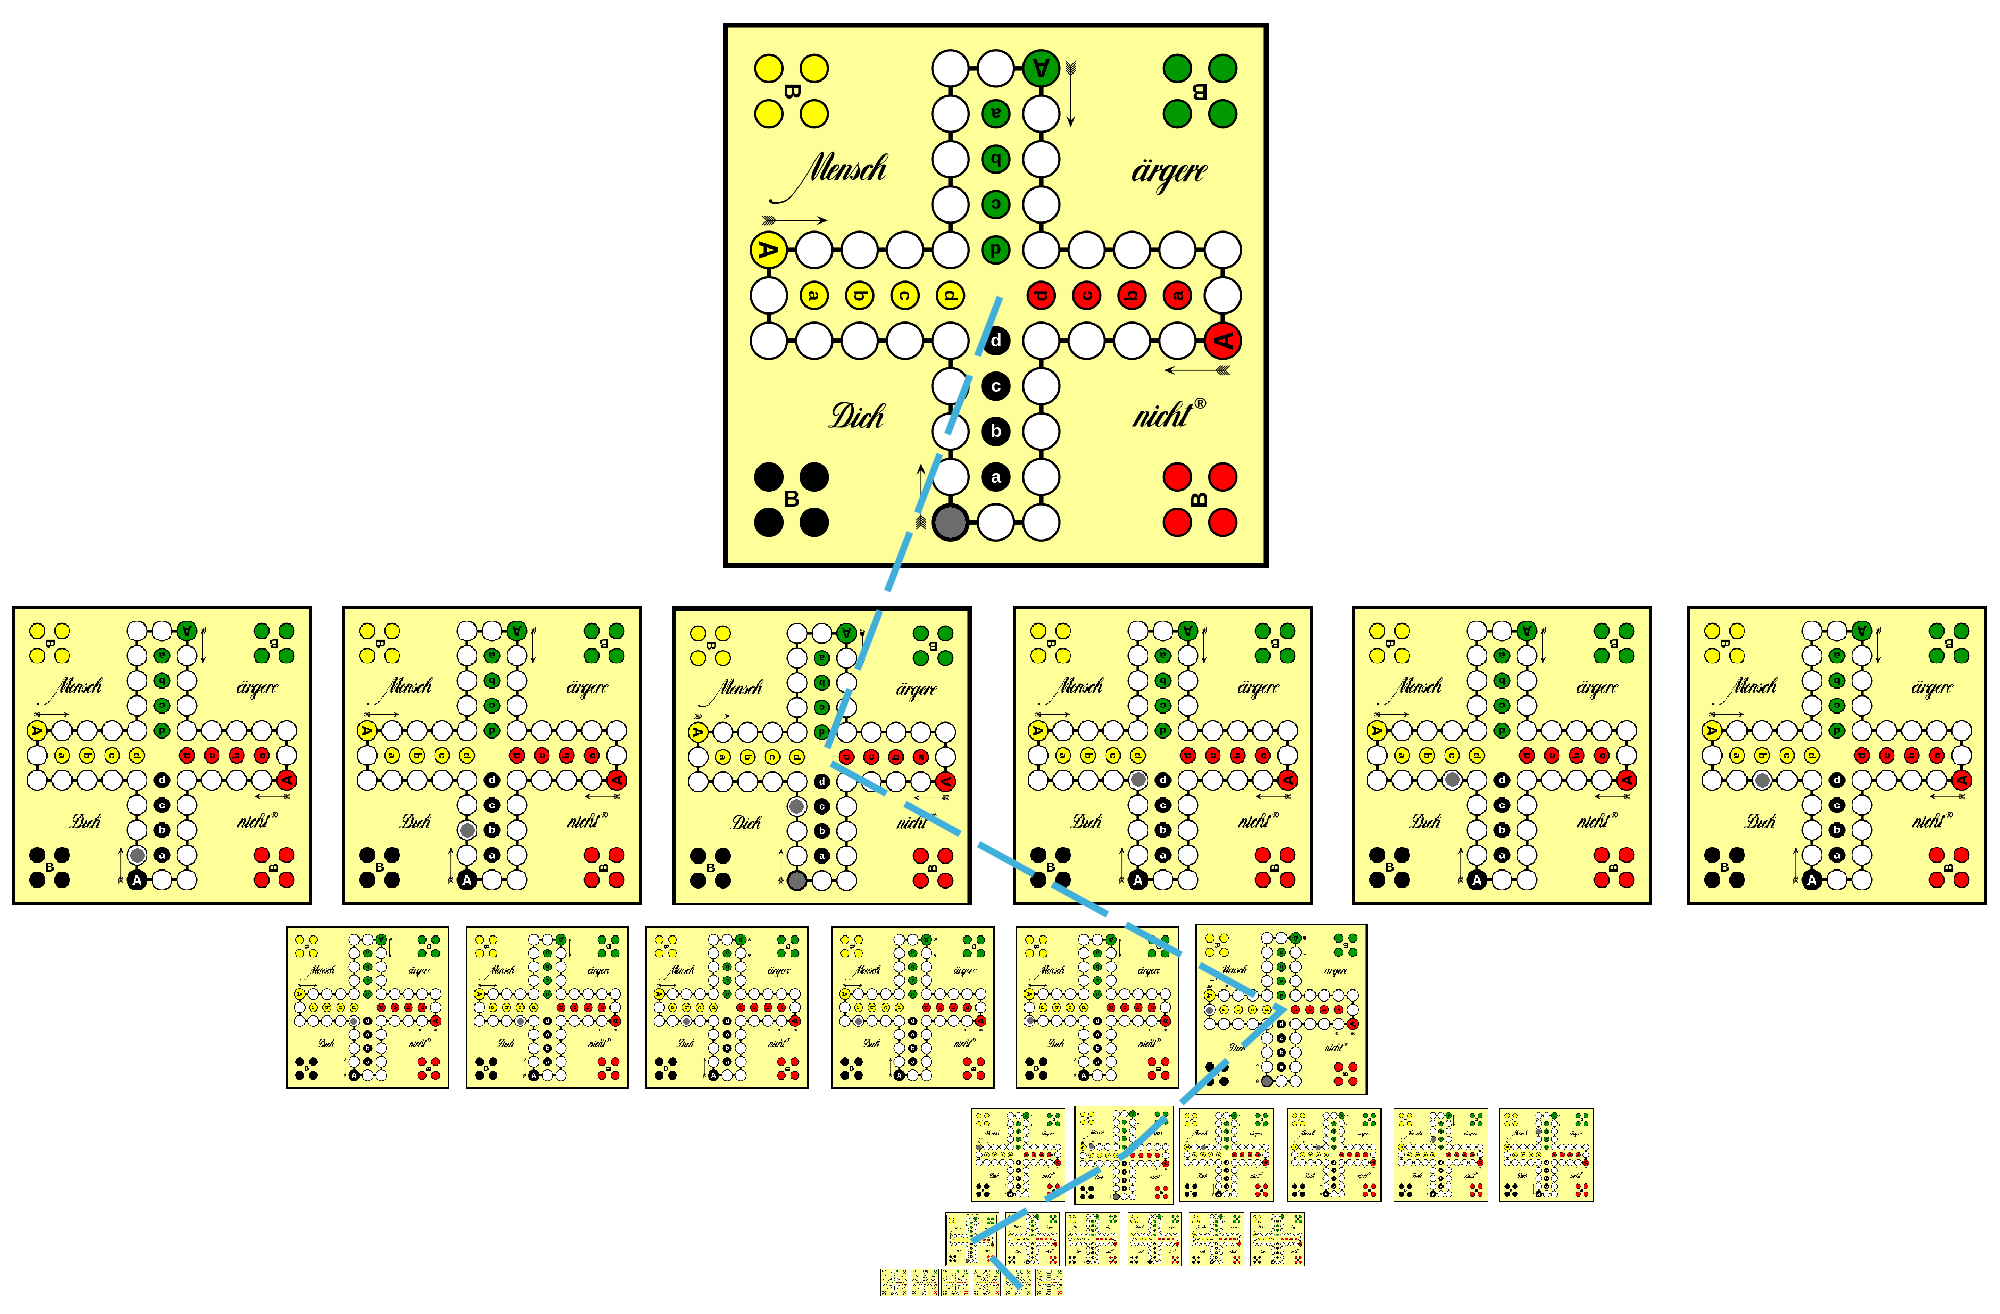
\includegraphics[width=1\textwidth]{images/Figure5}
    \caption{Singe path in tree}
    \label{fig:pathintree}
\end{figure}

The loop over the \textbf{sub-trees} of each position should start at 6 and count down. Rolling lower can only lead to shorter paths if it is not already possible to move to the goal in a straight line within one turn. Therefore, if a roll lands on the correct \textbf{abcd-tile} it is guaranteed that it will be the shortest path to goal from the current position. In that case any lower rolls and their \textbf{sub-trees} can be ignored.

Furthermore, the exploration of \textbf{sub-trees} can be halted if the current cumulative distance moved exceeds that of the shortest path identified thus far. Although there is no way to tell how many positions that will exclude ahead of time, it is definitely an essential part of optimization and could save billions of unnecessary calculations depending on how early the final shortest path is found.

There will be more specifics that become apparent as soon as we start implementing these concepts in code of course, but for now this should be a solid guideline for how to construct the program. But one more thing needs to be considered first.

\subsection{The bit-board}
We want to save the current position and the distance moved for every function call in the \textbf{position-tree}, however, as seen in Section 2 - Computability, that could take up an incredibly large amount of space if we are not careful with what data structure we choose.
There needs to be a way to save both position and distance in a relatively compact and fast but also still easy to understand way.

Ideally the function should only receive a single, non-pointer variable. That variable should also be fast at being read from or written to. 
Computer are very fast at doing \textbf{bitwise operations}, to the point where every other operation needs to be translated down into \textbf{bitwise operations}. If both position and distance could be saved in a single number that could then be modified and read from using \textbf{bitwise operators}, that structure would certainly satisfy our criteria.

A lot of the upcoming choices come down to personal preference. I have decided that I want a position to be represented by having each tile correspond to a bit. If the bit is a 0, it is empty. If it is a 1, there is a piece on the tile. From left to right the first 4 bits are the \textbf{purgatory}, the next 40 the main board and at the end there are 4 more bits for the \textbf{abcd-tiles}.
Since there are \textbf{48} relevant tiles, the use of a \textbf{32-bit} number is out of the question. Since the next higher standardized type is a \textbf{64-bit} number, we will have to stick with that, using the first \textbf{48} bits for the board state.

That leaves us with exactly \textbf{16} bits at the end. This space can be used for storing the amount of space moved up to the current position. Since we know every piece will receive it's own \textbf{bit-board} and thereby count only it's own movement, 16 bits are all we need. The distance between two tiles is \textbf{850} units while an \textbf{unsigned 16 bit integer} can represent numbers from \textbf{0} to \textbf{65536}.
\[
    Maximum~worst~case~tile ~movements = \frac{65536_{uint16~limit}}{850_{Board~side~length}} = 77.10117
\]
This means we can store the worst case zero shortcut movement over a board with almost twice the amount of tiles of the original board for every single piece. Therefore, as long as we stick to keeping distance counting separated between the pieces, there is no need to worry about running out of space.

Now we have a way to store all necessary information about a single position in the \textbf{position-tree} in a single number. If we want to store the entire movement across the board up to the current position, all we need to do is keep adding the new positions to the previous board, which means turning the new tile-bit to 1 one and not turning off the previous tile-bit. This means the board theoretically has more than 1 piece on the main-tiles at a time, but since there is no way to move backwards, the program will always know that the current piece is the rightmost of the pieces between the \textbf{purgatory} and the \textbf{abcd-tiles}. This is useful because it means we can not only represent a single state of the board, but the entire path of a single piece inside a 64-bit number.

Experimenting with \textbf{Visualizer.jar} or the \textbf{MaeDnVisualizer} directory helps with gaining an intuitive understanding of the structure of the \textbf{bit-board}.

\begin{figure}[htbp]
    \centering
    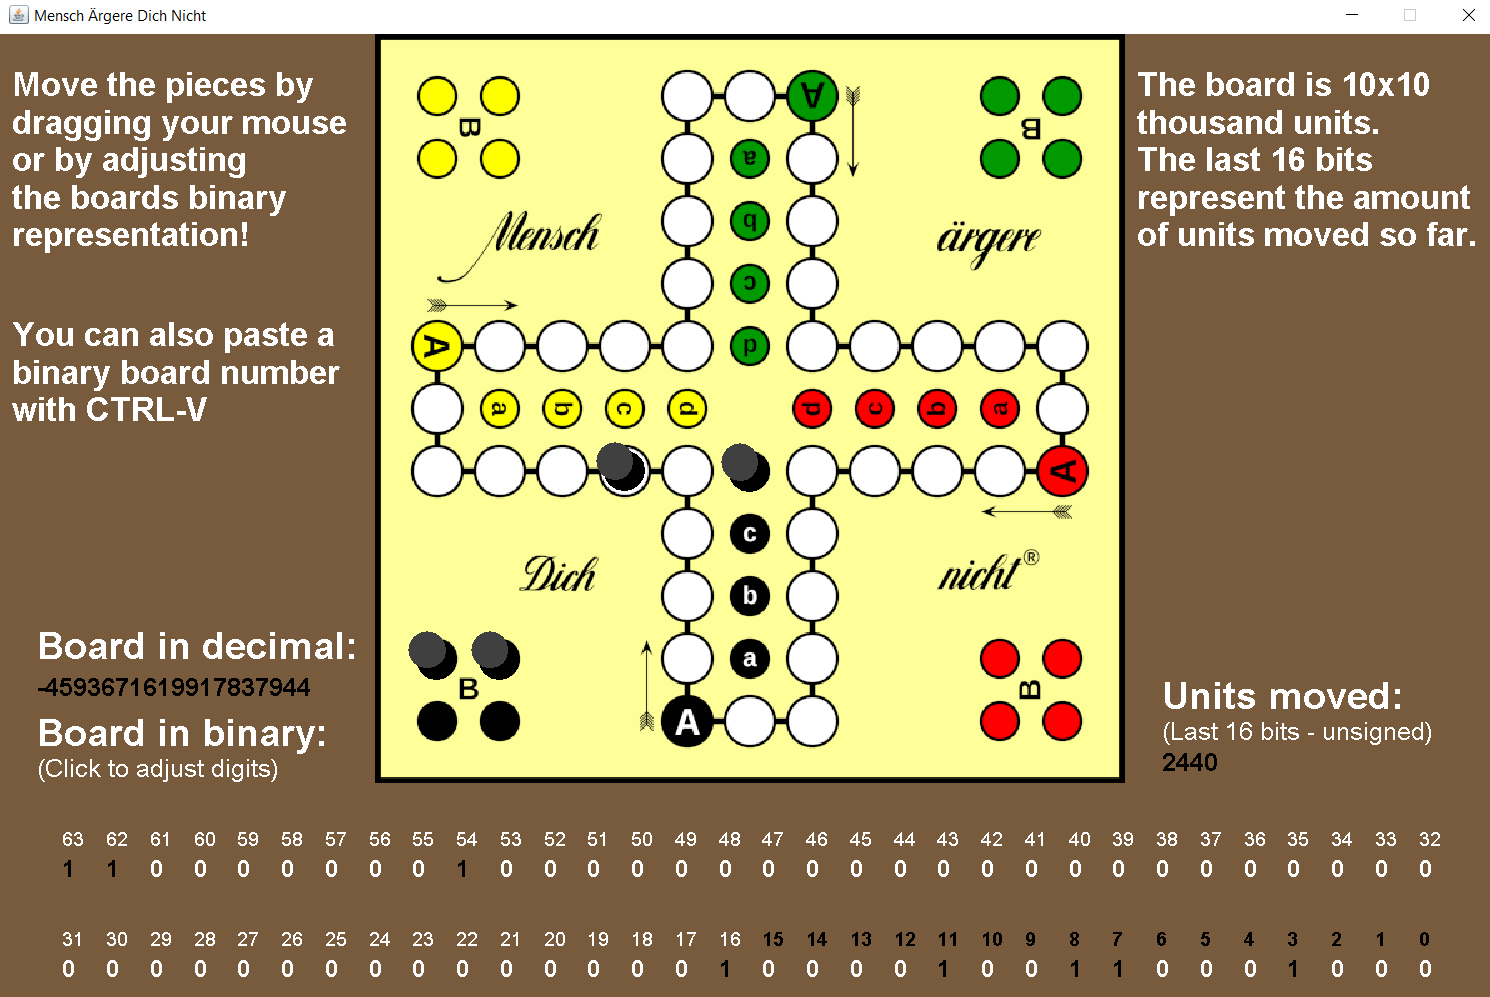
\includegraphics[width=0.9\textwidth]{images/Figure6}
    \caption{Visualizer.jar}
    \label{fig:visualizer}
\end{figure}

\newpage

\subsection{The code}

This section will focus on the specific implementation of the concepts discussed in the 3.1 and 3.2 in the C programming language.

Let us begin by defining a few constants.

\begin{lstlisting}[language=C, caption={Distance definitions}, label={lst:distance-defs}]

#define side_length_units 10000
#define tile_distance 850
#define min_units_per_tile 193 //best possible skip
#define start_pos_X 4170
#define start_pos_Y 9170
#define side_length_cm 36

\end{lstlisting}

4 out of these 6 have already been discussed previously. The definition for the side length in cm is going to be used for converting the unit length result into a result on an example board of 36cm x 36cm. The \textbf{min\_units\_per\_tile} definition will be used later, for now it is only important to know that it has been calculated by looking at the best possible skip on the board and dividing it's distance by the amount of tiles it covers.

The next set of definitions concerns the \textbf{bit-board}.

\begin{lstlisting}[language=C, caption={Bit-board definitions}, label={lst:bit-board-defs}]

#define starting_board 0b1111000000000000000000000000000000000000000000000000000000000000
#define start_p1 0b1110100000000000000000000000000000000000000000000000000000000000
#define start_p2 0b1100100000000000000000000000000000000000000000010000000000000000
#define start_p3 0b1000100000000000000000000000000000000000000000110000000000000000
#define start_p4 0b0000100000000000000000000000000000000000000001110000000000000000
#define distance_mask 0b0000000000000000000000000000000000000000000000001111111111111111
#define abcd_mask 0b0000000000000000000000000000000000000000000011110000000000000000
#define piece_extractor 0b0000111111111111111111111111111111111111111100000000000000000000
#define tile_40 0b0000000000000000000000000000000000000000000100000000000000000000
#define tile_1 0b0000100000000000000000000000000000000000000000000000000000000000
#define NULL_BOARD 0L

\end{lstlisting}

The meanings of these definitions can be guessed very well with an understanding of the \textbf{bit-board}. The \textbf{starting\_board} represents a board with 0 distance moved and all the pieces in \textbf{purgatory}.

The 4 starting position boards represent the positions in which all of the pieces begin their path. Note that the 16 distance bits are also 0 as each piece counts it's own and only it's own distance.
The main difference between the starting positions is the \textbf{purgatory} and the \textbf{abcd-tiles}. They are structured in a way were, in each turn, the rightmost bit in the \textbf{purgatory} is moved to the rightmost still empty \textbf{abcd-tile}. As discussed previously, this prevents pieces from getting in the way of each other.

The \textbf{distance\_mask} is \textbf{0} for every board bit and \textbf{1} for every distance bit. That means that the number representing only the distance moved can be extracted from any board simply by performing a \textbf{bitwise AND} operation with it and the \textbf{distance\_mask}. All the board-bits will be nullified and all the distance-bits keep their state.

The \textbf{abcd\_mask} and \textbf{piece\_extractor} work similarly. The first of which can be used to extract the finished pieces, the second of which extracts pieces that are on the board but neither in \textbf{purgatory} nor on the \textbf{abcd-tiles}.

The \textbf{tile\_40} and \textbf{tile\_1} masks should be self explanatory. However, their usefulness will only become apparent later.

The \textbf{NULL\_BOARD} is used to represent the end of a list of boards. It can safely be used as a stop-indicator because there is no position where there are zero pieces on the board.


The last important global declarations are the following:

\begin{lstlisting}[language=C, caption={Global declarations}, label={lst:global-declarations}]

static int64_t full_path[4] = {starting_board, NULL_BOARD, NULL_BOARD, NULL_BOARD};
static int full_path_index = 0;
static uint16_t cur_shortest = 0b1111111111111111; // distance in units

\end{lstlisting}

The \textbf{full\_path} array will be filled with the individual \textbf{bit-boards} representing the shortest path for each of the 4 pieces. The \textbf{full\_path\_index} will be used to address the correct position in the array. The \textbf{uint16\_t} variable \textbf{cur\_shortest} will be reset for every piece and is used to check, among other things, if a new found path should replace the previous one in the \textbf{full\_path} array because it is shorter.

With definitions and declarations out of the way, we can begin taking a look at the program structure, for which we will closely follow the order of execution. The \textbf{main()} method will get special treatment, as most of it is of little importance to this paper, like declaring a clock variable to measure the runtime or calling upon a method to convert the final result into cm.
Instead, the first important bit of code calls a function to calculate the distances between positions and store them in an array like discussed earlier, called \textbf{calculate\_distances()}.

\begin{lstlisting}[language=C, caption={Distance calculation}, label={lst:distance calculation}]

void calculate_distances()
{
    int from[2], to[2], vec[2];
    for (int i = 0; i < 40; i++)
    {
        get_coords(i, from);
        for (int j = 0; j < 6; j++)
        {
            get_coords(i+j+1, to);
            vec[0] = (int16_t) (to[0] - from[0]);
            vec[1] = (int16_t) (to[1] - from[1]);
            distances[i*6 + j] = round(sqrt(vec[0] * vec[0] + vec[1] * vec[1]));
        }
    }
}
\end{lstlisting}

The function loops over all 40 main-board spaces, whose coordinates are put into the array \textbf{from[]}, and calculates the distance to all 6 positions after it, which get their coordinates put into the array \textbf{to[]}. It does this by filling the \textbf{vec[]} array with the vector between both coordinates and that putting the length of that vector into the distance array. The array is global and it's size is 40 times 6, like discussed earlier in section 3.1. Multiplying i times 6 and adding j to it puts the distance in the right position in the array, as the layout inside is the following:
For each position the distances to the following 6 are stored in order, i.e. 1-2, 1-3, 1-4, 1-5, 1-6, 1-7, 2-3, 2-4....
\linebreak

The x and y coordinates are calculated using a function called \textbf{get\_coords()}.
\linebreak

\begin{lstlisting}[language=C, caption={Distance calculation}, label={lst:distance calculation}]

void get_coords(int index, int coords[])
{
    coords[0] = start_pos_X;
    coords[1] = start_pos_Y;


    //WALK ALONG GAME PATH
    int i = 0;
    while (i < index)
    {    
        if (i < 4) {coords[1] -= tile_distance;}
        else if (i < 8) {coords[0] -= tile_distance;}
        else if (i < 10) {coords[1] -= tile_distance;}
        else if (i < 14) {coords[0] += tile_distance;}
        else if (i < 18) {coords[1] -= tile_distance;}
        else if (i < 20) {coords[0] += tile_distance;}
        else if (i < 24) {coords[1] += tile_distance;}
        else if (i < 28) {coords[0] += tile_distance;}
        else if (i < 30) {coords[1] += tile_distance;}
        else if (i < 34) {coords[0] -= tile_distance;}
        else if (i < 38) {coords[1] += tile_distance;}
        else if (i < 39) {coords[0] -= tile_distance;}
        else {coords[1] -= tile_distance;}
        i++;
    }
}
\end{lstlisting}

This is not the most ideal way to handle the problem, but it is fast and simple. All the function does is start at the starting coordinates that have been defined earlier and then follow the path of the board, adding the distance between tiles each time. We begin by moving up (y is decreasing) 4 times, then we move to the left (x is decreasing), then up again and so on across the entire board.
Consider the following tile indices:

\begin{figure}[htbp]
    \centering
    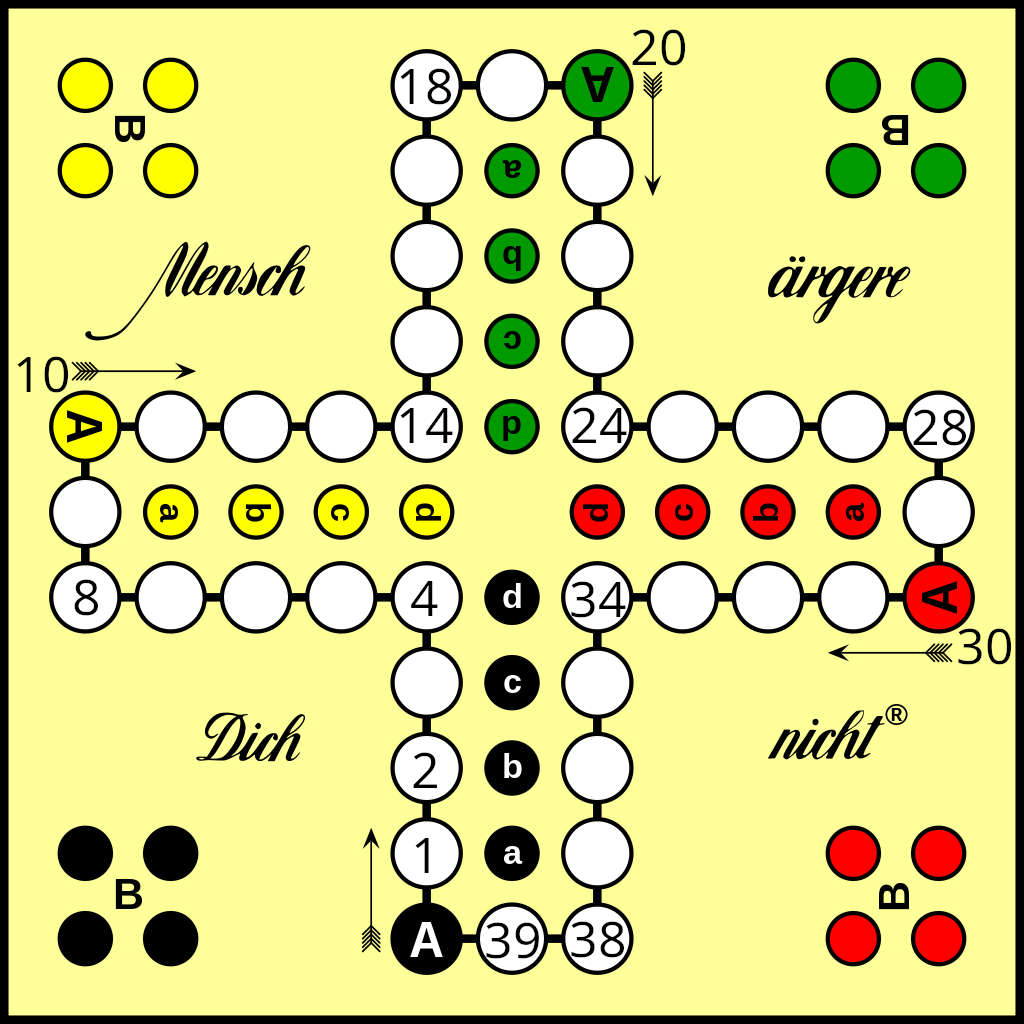
\includegraphics[width=0.4\textwidth]{images/Figure7}
    \caption{Tile indices}
    \label{fig:tile-indices}
\end{figure}

\newpage

Now that the distances have been pre-calculated, the main loop function, \textbf{find\_shortest\_path()}, is called.

\begin{lstlisting}[language=C, caption={Find shortest path}, label={lst:find-shortest-path}]

int find_shortest_path()
{
    int path_length = total_movement_to_A;

    int64_t start_board;
    while (full_path_index < 4)
    {
        switch (full_path_index)
        {
            case 0: start_board = start_p1;break;
            case 1: start_board = start_p2; break;
            case 2: start_board = start_p3; break;
            case 3: start_board = start_p4; break;
            default: break;
        }
        handle_piece(start_board);
        path_length += cur_shortest;
        cur_shortest = distance_mask; //RESET
        full_path_index++;
    }

    return path_length;
}
\end{lstlisting}

The main core of the function revolves around calling a separate function to handle each of the 4 single pieces in a loop, adding the therein calculated shortest path to the total path length and then resetting the global \textbf{cur\_shortest} variable for the next piece. The total path length is then returned at the end. At the start the path length is initialized to have the value \textbf{total\_movement\_to\_A} which is the constant calculated in section 3.1 that represents the minimum amount of movement needed for all 4 pieces to get to their starting positions. The \textbf{start\_board} that is passed to the \textbf{handle\_piece} function is initialized at the starting position of every piece, so it is necessary to add this constant as it will not be calculated as part of the path.

\newpage

Now let us take a look at by far the most important function in this algorithm, \textbf{handle\_piece()}.

\begin{lstlisting}[language=C, caption={Handle piece}, label={lst:handle-piece}]

void handle_piece(int64_t path)
{
    int64_t piece_mask = extract_piece(path, EXTRACT_RIGHTMOST);

    //CHECK IF PATH CAN EVEN STILL BE SHORTER THAN cur_shortest
    int tiles_left = 0;
    int64_t temp_piece_mask = piece_mask;
    while(!(temp_piece_mask&(path&abcd_mask|distance_mask)))
    {
        temp_piece_mask >>= 1;
        tiles_left++;
    }
    tiles_left--;

    if ((path & distance_mask) + tiles_left*min_units_per_tile  > cur_shortest)
    {return;}

    for (int i = 6; i > 0; i--)
    {
        int64_t roll = piece_mask >> i;

        // skip if roll enters last 16 bits or lands on a finished piece
        if ((roll & (distance_mask|path))) {continue;}

        int dist = get_distance(piece_mask, i);

        if (roll & abcd_mask)
        {
            //Check if roll lands on the rightmost empty position
            if ((roll >> 1) & (path|distance_mask))
            {
                int new_length = (int) (path & distance_mask) + dist;

                if (new_length < cur_shortest)
                {
                    full_path[full_path_index] = (path | roll) + dist;
                    cur_shortest = new_length;
                }
                return;
            }
        }
        else
        {
            handle_piece((path | roll) + dist); //Handle current rolls subtree
        }
    }
}
\end{lstlisting}

At the very start the function \textbf{extract\_piece()} is called with the parameters \textbf{path} and \textbf{EXTRACT\_RIGHTMOST}. This function should take the \textbf{path bit-board} and return a \textbf{bit-board} containing only the rightmost, non-finished piece on the board and then store it in \textbf{piece\_mask}.

This is how the program extracts the rightmost of leftmost piece:

\begin{lstlisting}[language=C, caption={Extract piece}, label={lst:extract-piece}]
int64_t extract_piece(int64_t path, int operation_flag)
{
    int64_t piece_mask = path & piece_extractor;
    if (piece_mask == NULL_BOARD) {return NULL_BOARD;}

    int64_t extracted;

    if (operation_flag == EXTRACT_RIGHTMOST)
    {
        extracted = tile_40;
        while (!(extracted&piece_mask)) {extracted <<= 1;}
    }

    else
    {
        extracted = tile_1;
        while (!(extracted&piece_mask)) {extracted >>= 1;}
    }

    return extracted;
}
\end{lstlisting}

First, a \textbf{piece\_mask} is created through a \textbf{bitwise AND} with the \textbf{piece\_extractor} mask defined earlier. Now that variable stores a board with only the pieces on the main 40 tiles. A piece is extracted by creating a \textbf{bit-board} called \textbf{extracted} with all zeros except for a single one at either the start (\textbf{tile\_1}) or the end (\textbf{tile\_40}) of the main-board. If we want to extract the rightmost piece, \textbf{extracted} is \textbf{bit-shifted} to the left, and otherwise to the right, until it overlaps with the \textbf{piece\_mask}. That means \textbf{extracted} is at the position of either the rightmost or leftmost piece on the given board and can be returned.

\newpage

Now let us return to the \textbf{handle\_piece()} function. After the rightmost piece - which represents the piece the function currently needs to work with - is retrieved, the following sub-task is executed:


\begin{lstlisting}[language=C, caption={Return condition}, label={lst:return-condition}]
//CHECK IF PATH CAN EVEN STILL BE SHORTER THAN cur_shortest
int tiles_left = 0;
int64_t temp_piece_mask = piece_mask;
while(!(temp_piece_mask&(path&abcd_mask|distance_mask)))
{
    temp_piece_mask >>= 1;
    tiles_left++;
}
tiles_left--;

if ((path & distance_mask) + tiles_left*min_units_per_tile  > cur_shortest)
{return;}

\end{lstlisting}

The purpose of this sub-task is to make an estimation of how many units, at bare minimum, are left until the goal. First it calculates the amount of tiles left. That can be done similarly to how the \textbf{extract\_piece()} function operates but performing a \textbf{bitwise AND} check with a combination of \textbf{path}, \textbf{abcd\_mask} and \textbf{distance\_mask} instead. The result of combining these three with a \textbf{bitwise AND} and a \textbf{bitwise OR} is a \textbf{bit-board} that is all zeros except for the pieces that were already on the \textbf{abcd-tiles} and the 16 distance bits. If the temporary \textbf{piece\_mask} intersects that \textbf{bit-board} we know it has passed the rightmost still empty position and we can stop counting.
The amount of distance left is calculated by multiplying the tiles left with the \textbf{min\_units\_per\_tile} constant we defined earlier. If the current distance plus the minimum distance left is already longer than the \textbf{cur\_shortest} path, we know searching any deeper in this \textbf{sub-tree} is useless and can return.
\linebreak

The final part of the \textbf{handle\_piece()} function is a loop over all 6 different rolls from the current position wherein the function calls itself recursively with the newly rolled position. Recall that we start the loop at 6 and count downwards to decrease the chance of unnecessarily going into \textbf{sub-trees} that would be cut off if a higher roll finishes more quickly anyway.
First, a \textbf{bit-board} called \textbf{roll} is defined, which is simply the \textbf{piece\_mask} from earlier \textbf{bit-shifted} i times to the right. In other words, it is a \textbf{bit-board} in which the current piece was moved to the right by an amount of tiles equal to the currently rolled number that is being checked.

\begin{lstlisting}[language=C, caption={Roll loop}, label={lst:roll-loop}]

 for (int i = 6; i > 0; i--)
    {
        int64_t roll = piece_mask >> i;

        // skip if roll enters last 16 bits or lands on a finished piece
        if ((roll & (distance_mask|path))) {continue;}

        int dist = get_distance(piece_mask, i);

        if (roll & abcd_mask)
        {
            //Check if roll lands on the rightmost empty position
            if ((roll >> 1) & (path|distance_mask))
            {
                int new_length = (int) (path & distance_mask) + dist;

                if (new_length < cur_shortest)
                {
                    full_path[full_path_index] = (path | roll) + dist;
                    cur_shortest = new_length;
                }
                return;
            }
        }
        else
        {
            handle_piece((path | roll) + dist); //Handle current rolls subtree
        }
    }

\end{lstlisting}

Then, we check whether the roll is even valid. If it's \textbf{bit-board} intersects with the path we know it landed on a finished piece and if it intersects with the \textbf{distance\_mask} we know it has left the bounds of the board. In such a case the roll is simply skipped.
Next we retrieve the distance between the current position and the current roll and store it in \textbf{dist}. How exactly that is done will be shown later. If the result of a \textbf{bitwise AND} between "roll" and \textbf{abcd\_mask} is positive, we need to check if the piece has landed on the rightmost still empty \textbf{abcd-tile}. That is the case when the roll \textbf{bit-shifted} 1 to the right intersects path or the \textbf{distance\_mask}. This sort of check only works if we checked the roll for validity earlier. If we now know that the piece has finished, we can calculate the length of this path by adding \textbf{dist} to the distance extracted from "path" using the \textbf{distance\_mask}. If that new length is less than that of the \textbf{cur\_shortest} path, it becomes the new shortest and is stored in the \textbf{full\_path} array. Now we can return.

If the piece has not finished however, we need to search it's \textbf{sub-trees}. For that we call \textbf{handle\_piece()} recursively and pass in a new \textbf{bit-board} with the new roll inserted through \textbf{bitwise OR} and the new distance added on top.
This way, the function should eventually go through every relevant \textbf{sub-tree} one by one, cutting of all \textbf{sub-trees} with no chance of getting a shorter path and should thereby eventually finish with the shortest overall path stored in the \textbf{full\_path} array.


The function to retrieve the distance between to positions from the array, \textbf{get\_distance()}, might seem a bit odd at first:

\begin{lstlisting}[language=C, caption={Get distance}, label={lst:get-distance}]

int get_distance(int64_t from, int roll_num)
{
    int from_index = 0;
    while(!(from & starting_board))
    {
        from <<= 1;
        from_index++;
    }
    from_index--;

    int distance = distances[from_index * 6 + (roll_num-1)];
    return distance;
}
\end{lstlisting}

The actual retrieval is easy, you simply get the value from the array at the correct position corresponding to how we set up the distances array earlier. But getting the index in the board of the piece in the \textbf{bit-board} "from" is a bit more difficult. Luckily, the \textbf{bit-board} passed into the function is always one that has been through the \textbf{piece\_mask}, meaning it is all zeros except for a single 1. That means that the index can be obtained by \textbf{bit-shifting} the board to the left until it overlaps with the starting board, checked through \textbf{bitwise AND}. We simply keep track of how often we need to shift and then remove the last shift that ended up overlapping to get the correct index.

There are more functions related to printing, timing and converting units, but they are not important to this paper. The functions discussed here are enough to lead us to the result.

\section{Discussion}

\subsection{Results}

The shortest path on a 10,000x10,000 unit board is \textbf{83047 units} long.
On a 36x36 cm board that is is \textbf{298.9692 cm}.
That is almost twice the circumference. But the length is mostly meaningless. More importantly, what does that path look like?

Well, here it is:


(If you would like to see the bit representation of this path, simply run the \textbf{brute\_forcer.c} file. Each individual \textbf{bit-board} can then be copied and pasted into \textbf{Visualizer.jar} to get this exact result.)

\begin{figure}[htbp]
    \centering
    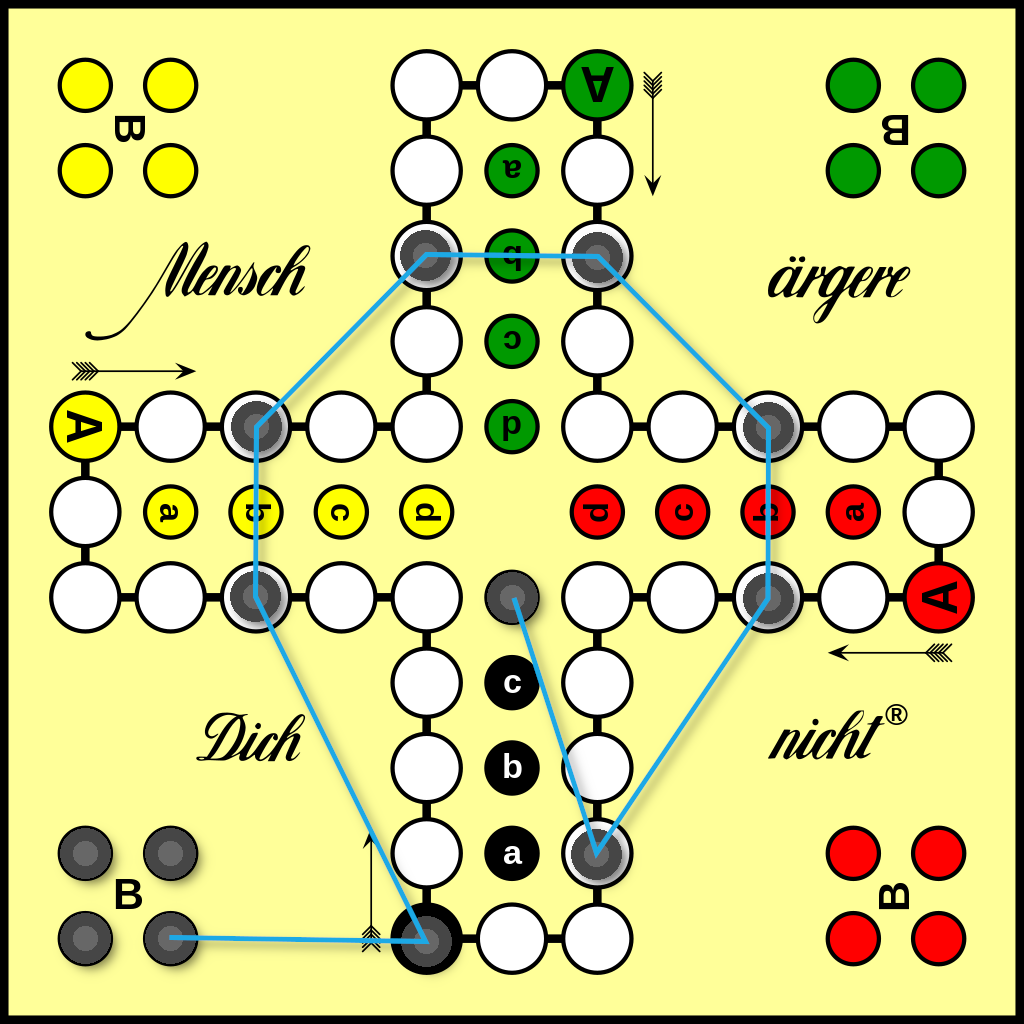
\includegraphics[width=0.6\textwidth]{images/Figure8}
    \caption{Piece 1 - 19462 units}
    \label{fig:piece1}
\end{figure}

\begin{figure}[htbp]
    \centering
    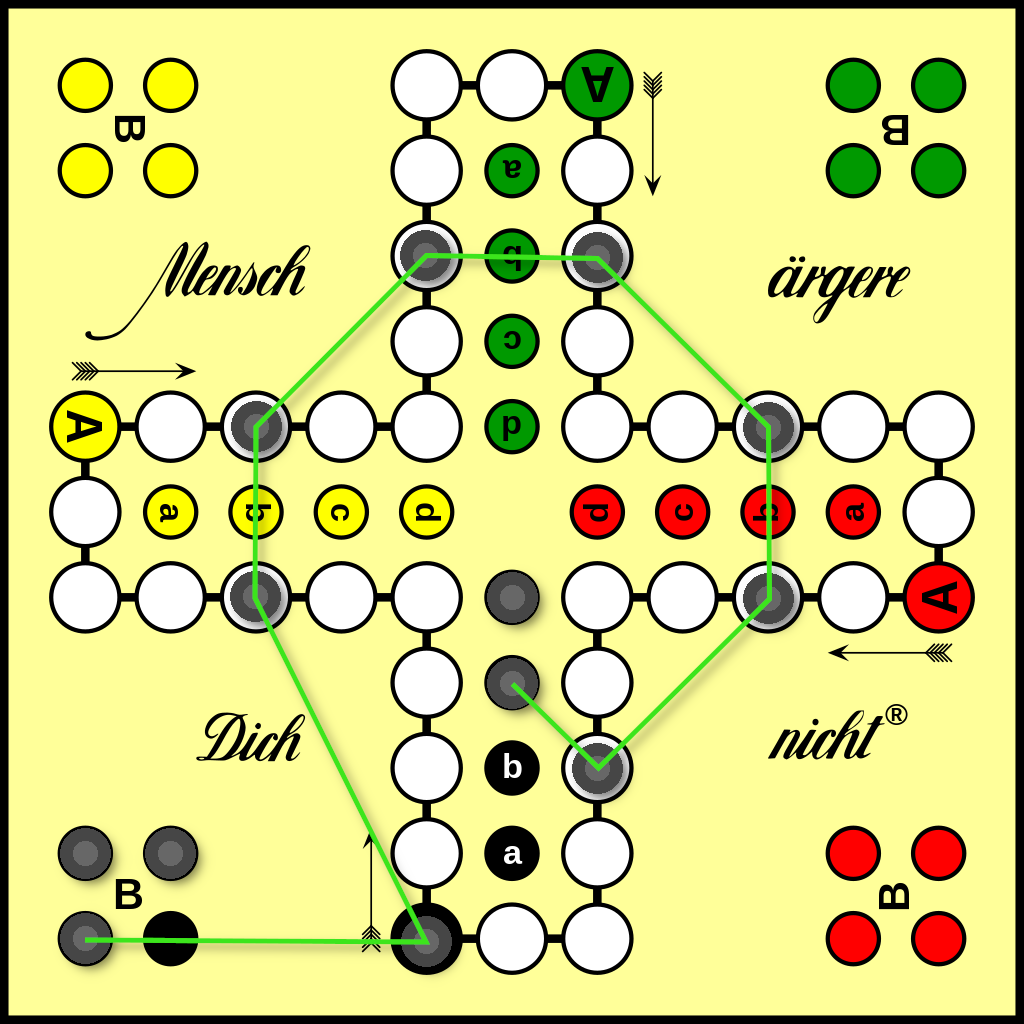
\includegraphics[width=0.6\textwidth]{images/Figure9}
    \caption{Piece 2 - 17315 units}
    \label{fig:piece2}
\end{figure}

\begin{figure}[htbp]
    \centering
    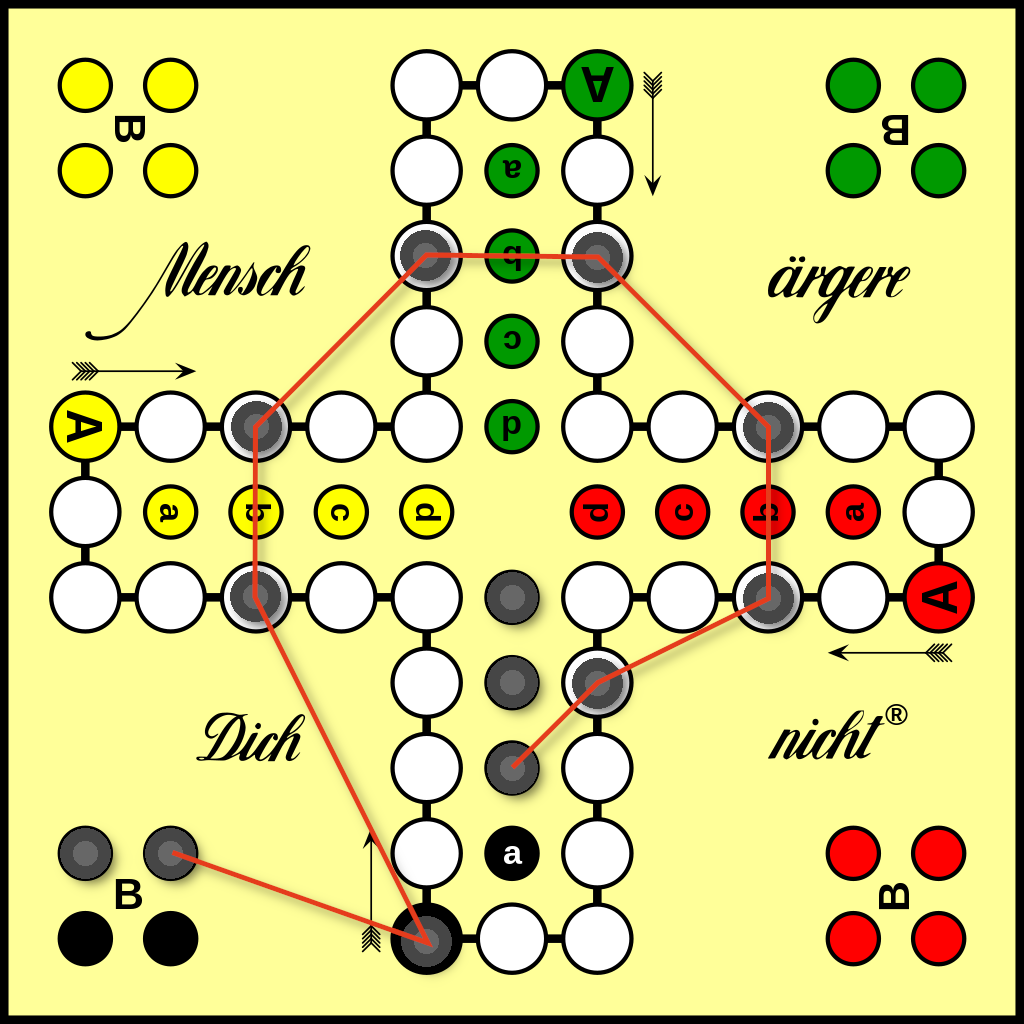
\includegraphics[width=0.6\textwidth]{images/Figure10}
    \caption{Piece 3 - 16812 units}
    \label{fig:piece3}
\end{figure}

\begin{figure}[htbp]
    \centering
    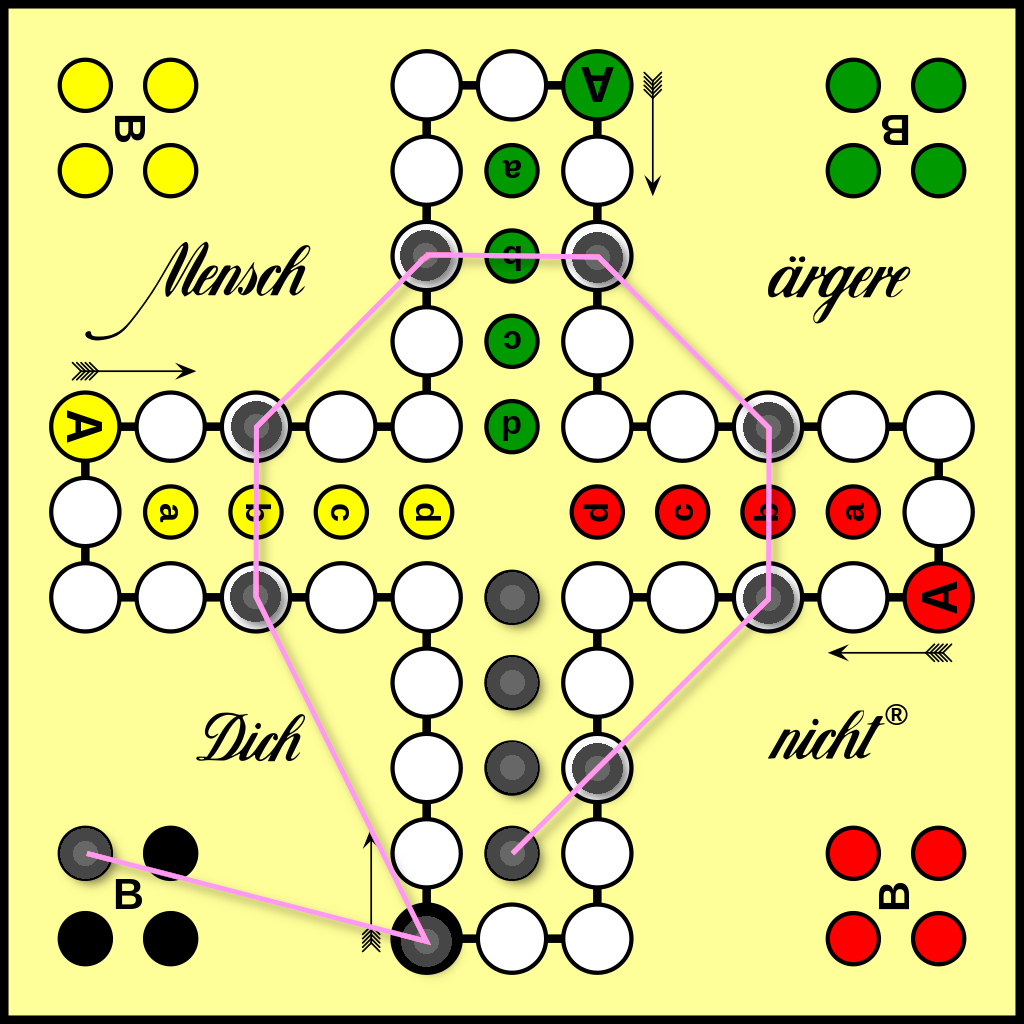
\includegraphics[width=0.6\textwidth]{images/Figure11}
    \caption{Piece 4 - 17315 units}
    \label{fig:piece4}
\end{figure}

\begin{figure}[htbp]
    \centering
    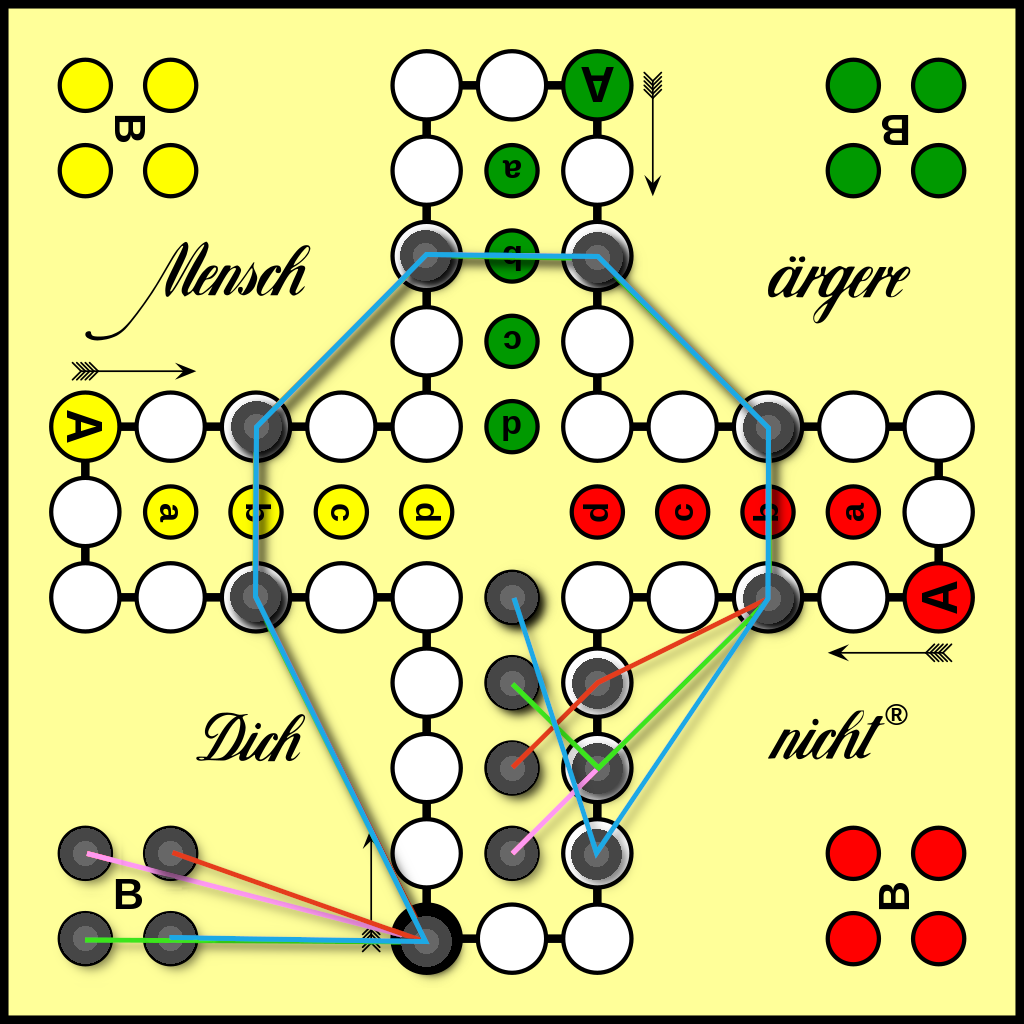
\includegraphics[width=0.6\textwidth]{images/Figure12}
    \caption{Full path - 83047 units}
    \label{fig:full-path}
\end{figure}

\newpage
Interestingly, the paths only differ at two parts of the board. The first of which is obvious. The pieces start at different positions but are required to move to the starting position A when exiting purgatory. The other point where the paths differ is at the last two rolls. Since the pieces end goals are different, there will of course be different ideal paths. \textbf{Piece 1 (blue)} needs to make quite a sharp turn at the end to reach to furthest back \textbf{abcd-tile}. Meanwhile, \textbf{piece 4 (pink)} can go in a perfectly straight path from the position where the paths diverge to it's end goal. However, the shortest singular path is actually \textbf{piece 3 (red)}, even though it cannot move in a straight line at the end like \textbf{piece 4 (pink)}. That is due to two reasons. The first of which being that \textbf{red} starts of one tile closer to the starting position than \textbf{pink}. Secondly, while pink may be able to move in a straight line, red's goal is actually closer to the divergence point.

The 6 rolls in which all paths are equal are also quite interesting. A sequence of rolls \textbf{6-6-6-4-6-4-6} (including the 6 required to exit the \textbf{purgatory}) One the one hand this clearly shows that the highest roll is not always the optimal one, but on the other hand it is also clear that rolling higher is generally better. This reinforces our prior choice to loop over \textbf{sub-trees} starting from higher rolls to cut off unnecessary branches more quickly.

All of the single piece paths require exactly \textbf{9} rolls when including the 6 rolled to exit the \textbf{purgatory}. That means the entire path requires \textbf{36} rolls.

Because we know the rolls are equal until the very last 2, the average roll in the entire path can be calculated very quickly.

\begin{align*}
    \text{Roll total} &= 4 \cdot \left( 6+6+6+4+6+4+6 \right)_{\text{Overlap}} \\
    &\quad + \left( 5+6 \right)_{\text{Piece 1}} + \left( 4+6 \right)_{\text{Piece 2}} \\
    &\quad + \left( 3+6 \right)_{\text{Piece 3}} + \left( 4+4 \right)_{\text{Piece 4}} = 190
\end{align*}

\[
	\text{Average roll} =  \frac{\text{Roll total}}{\text{Roll count}} = \frac{190}{36} \approx 5.27
\]

Close to 6, but still showing that 6 is not \textbf{always} the ideal roll.

\newpage

Lastly, here are the absolute and relative totals of each roll in the final path:

\begin{itemize}
    \item \textbf{1} - Rolled \textbf{0} times. \textbf{0\%} of all rolls.
    \item \textbf{2} - Rolled \textbf{0} times. \textbf{0\%} of all rolls.
    \item \textbf{3} - Rolled \textbf{1} time. \textbf{2.78\%} of all rolls
    \item \textbf{4} - Rolled \textbf{11} times. \textbf{33.55\%} of all rolls.
    \item \textbf{5} - Rolled \textbf{1} time. \textbf{2.78\%} of all rolls.
    \item \textbf{6} - Rolled \textbf{23} times. \textbf{63.89\%} of all rolls.
\end{itemize}

\begin{figure}[htbp]
    \centering
    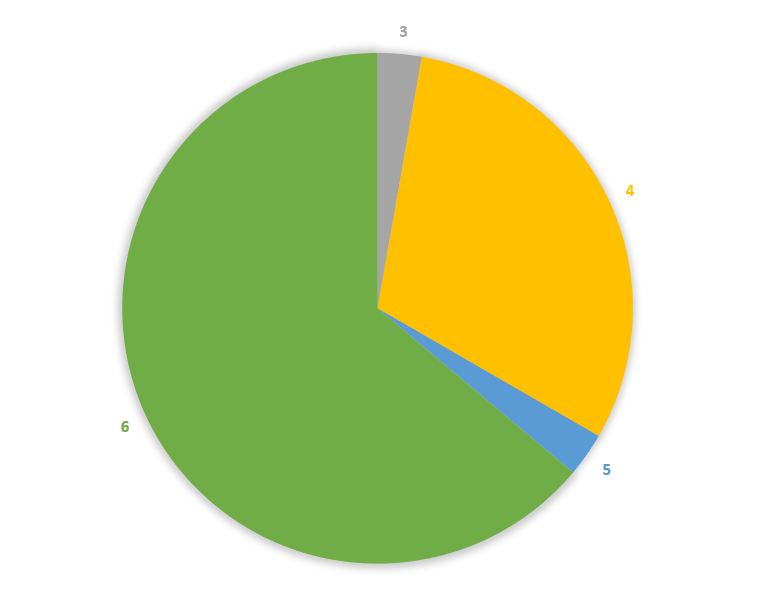
\includegraphics[width=1\textwidth]{images/Figure13}
    \caption{Roll diagram}
    \label{fig:roll-diagram}
\end{figure}

\subsection{Runtime}

In the final version of the program, the \textbf{handle\_piece()} function is called \linebreak \textbf{18 526 851} times in total. Of which \textbf{15 422 842} calls are immediately cut short because it has been calculated that their \textbf{sub-trees} have no chance of beating the current shortest path. That is quite remarkable. More than \textbf{83\%} of all calls to the function end up getting cut short. 

\begin{figure}[htbp]
    \centering
    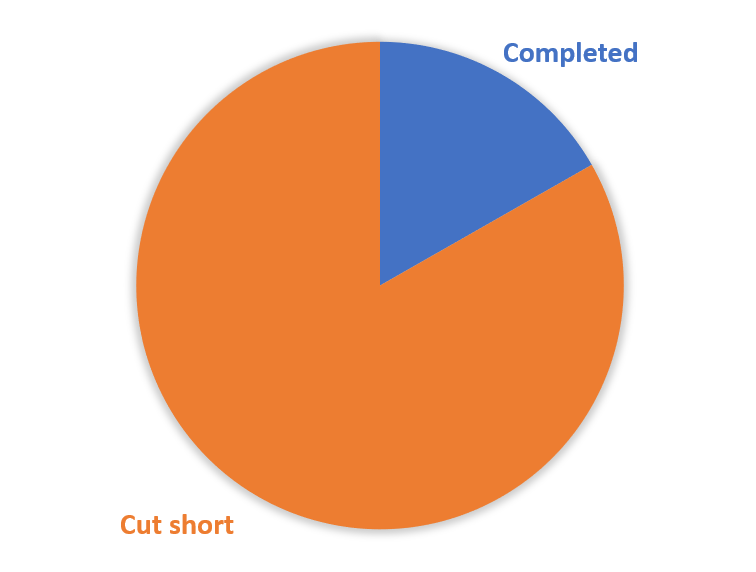
\includegraphics[width=0.4\textwidth]{images/Figure14}
    \caption{Total optimized function calls}
    \label{fig:func-call-diagram-1}
\end{figure}

Clearly, that little check is quite the time saver. If we only check for whether or not the current distance is already longer than the shortest path and omit the \textbf{min\_distance\_per\_tile} calculation, the function is called \textbf{660 449 985} times. Such a small calculation saves us \textbf{97\%} of these function calls.

\begin{figure}[htbp]
    \centering
    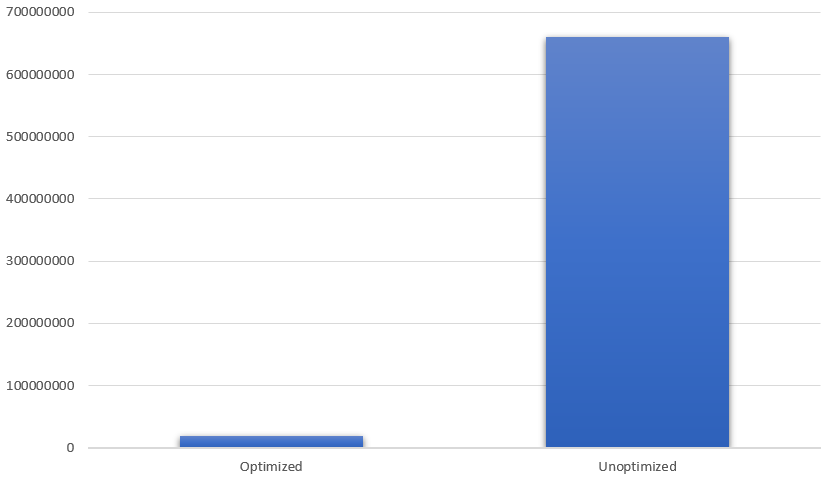
\includegraphics[width=0.73\textwidth]{images/Figure15}
    \caption{Total function calls compared}
    \label{fig:func-call-diagram-2}
\end{figure}

\newpage

The algorithm has an average runtime of \textbf{0.5 seconds} on my \textit{AMD Ryzen 9 5950x} CPU. This is quite remarkable when compared to the numbers calculated in Section 2 - Computability. However, exiting a branch once it has been calculated that there can no longer be a shorter path than the current shortest in this branch by using the  \text{min\_units\_per\_square} constant could be considered cheating. After all, there was no way for me to be fully confident in it's validity before running the program.
If we take out that optimization the program calls the function  times and runs for \textbf{22 seconds}.

These are the three functions that take up the majority of the runtime:

\begin{itemize}
	\item \textbf{extract\_piece()} 15\%
	\item \textbf{handle\_piece()} 25\%
	\item \textbf{get\_distance()} 60\%
\end{itemize}

\begin{figure}[htbp]
    \centering
    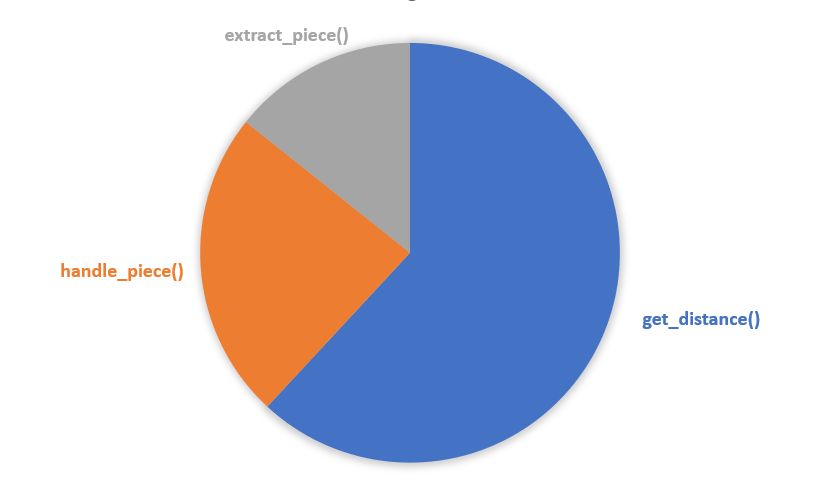
\includegraphics[width=0.8\textwidth]{images/Figure16}
    \caption{Total runtime}
    \label{fig:runtime-diagram}
\end{figure}

It seems the majority of the time is spent looking up distances in the pre-calculated distances array. However, it is important to remember that \textbf{get\_distance()} also handles finding the index of the current piece on it's own. More importantly, being inside the loop over all 6 rolls in \textbf{handle\_piece()}, \textbf{get\_distance()} is called a lot more often than the other two functions.


\end{document}